\documentclass[twoside]{book}

% Packages required by doxygen
\usepackage{fixltx2e}
\usepackage{calc}
\usepackage{doxygen}
\usepackage[export]{adjustbox} % also loads graphicx
\usepackage{graphicx}
\usepackage[utf8]{inputenc}
\usepackage{makeidx}
\usepackage{multicol}
\usepackage{multirow}
\PassOptionsToPackage{warn}{textcomp}
\usepackage{textcomp}
\usepackage[nointegrals]{wasysym}
\usepackage[table]{xcolor}

% Font selection
\usepackage[T1]{fontenc}
\usepackage[scaled=.90]{helvet}
\usepackage{courier}
\usepackage{amssymb}
\usepackage{sectsty}
\renewcommand{\familydefault}{\sfdefault}
\allsectionsfont{%
  \fontseries{bc}\selectfont%
  \color{darkgray}%
}
\renewcommand{\DoxyLabelFont}{%
  \fontseries{bc}\selectfont%
  \color{darkgray}%
}
\newcommand{\+}{\discretionary{\mbox{\scriptsize$\hookleftarrow$}}{}{}}

% Page & text layout
\usepackage{geometry}
\geometry{%
  a4paper,%
  top=2.5cm,%
  bottom=2.5cm,%
  left=2.5cm,%
  right=2.5cm%
}
\tolerance=750
\hfuzz=15pt
\hbadness=750
\setlength{\emergencystretch}{15pt}
\setlength{\parindent}{0cm}
\setlength{\parskip}{3ex plus 2ex minus 2ex}
\makeatletter
\renewcommand{\paragraph}{%
  \@startsection{paragraph}{4}{0ex}{-1.0ex}{1.0ex}{%
    \normalfont\normalsize\bfseries\SS@parafont%
  }%
}
\renewcommand{\subparagraph}{%
  \@startsection{subparagraph}{5}{0ex}{-1.0ex}{1.0ex}{%
    \normalfont\normalsize\bfseries\SS@subparafont%
  }%
}
\makeatother

% Headers & footers
\usepackage{fancyhdr}
\pagestyle{fancyplain}
\fancyhead[LE]{\fancyplain{}{\bfseries\thepage}}
\fancyhead[CE]{\fancyplain{}{}}
\fancyhead[RE]{\fancyplain{}{\bfseries\leftmark}}
\fancyhead[LO]{\fancyplain{}{\bfseries\rightmark}}
\fancyhead[CO]{\fancyplain{}{}}
\fancyhead[RO]{\fancyplain{}{\bfseries\thepage}}
\fancyfoot[LE]{\fancyplain{}{}}
\fancyfoot[CE]{\fancyplain{}{}}
\fancyfoot[RE]{\fancyplain{}{\bfseries\scriptsize Generated by Doxygen }}
\fancyfoot[LO]{\fancyplain{}{\bfseries\scriptsize Generated by Doxygen }}
\fancyfoot[CO]{\fancyplain{}{}}
\fancyfoot[RO]{\fancyplain{}{}}
\renewcommand{\footrulewidth}{0.4pt}
\renewcommand{\chaptermark}[1]{%
  \markboth{#1}{}%
}
\renewcommand{\sectionmark}[1]{%
  \markright{\thesection\ #1}%
}

% Indices & bibliography
\usepackage{natbib}
\usepackage[titles]{tocloft}
\setcounter{tocdepth}{3}
\setcounter{secnumdepth}{5}
\makeindex

% Hyperlinks (required, but should be loaded last)
\usepackage{ifpdf}
\ifpdf
  \usepackage[pdftex,pagebackref=true]{hyperref}
\else
  \usepackage[ps2pdf,pagebackref=true]{hyperref}
\fi
\hypersetup{%
  colorlinks=true,%
  linkcolor=blue,%
  citecolor=blue,%
  unicode%
}

% Custom commands
\newcommand{\clearemptydoublepage}{%
  \newpage{\pagestyle{empty}\cleardoublepage}%
}

\usepackage{caption}
\captionsetup{labelsep=space,justification=centering,font={bf},singlelinecheck=off,skip=4pt,position=top}

%===== C O N T E N T S =====

\begin{document}

% Titlepage & ToC
\hypersetup{pageanchor=false,
             bookmarksnumbered=true,
             pdfencoding=unicode
            }
\pagenumbering{roman}
\begin{titlepage}
\vspace*{7cm}
\begin{center}%
{\Large E\+D\+DL Parser }\\
\vspace*{1cm}
{\large Generated by Doxygen 1.8.11}\\
\end{center}
\end{titlepage}
\clearemptydoublepage
\tableofcontents
\clearemptydoublepage
\pagenumbering{arabic}
\hypersetup{pageanchor=true}

%--- Begin generated contents ---
\chapter{E\+D\+DL Parser}
\label{index}\hypertarget{index}{}This is a very basic E\+D\+DL parser used for a proof of concept. May be expanded in the future. 
\chapter{Class Index}
\section{Class List}
Here are the classes, structs, unions and interfaces with brief descriptions\+:\begin{DoxyCompactList}
\item\contentsline{section}{\hyperlink{structeddl__object}{eddl\+\_\+object} }{\pageref{structeddl__object}}{}
\item\contentsline{section}{\hyperlink{structeddl__variable}{eddl\+\_\+variable} }{\pageref{structeddl__variable}}{}
\end{DoxyCompactList}

\chapter{File Index}
\section{File List}
Here is a list of all documented files with brief descriptions\+:\begin{DoxyCompactList}
\item\contentsline{section}{/home/alxhoff/git/\+E\+D\+D\+L-\/parser/\+E\+D\+D\+L-\/\+Parser/\hyperlink{eddl__data__type_8h}{eddl\+\_\+data\+\_\+type.\+h} \\*Text parser to extract information from E\+DD files }{\pageref{eddl__data__type_8h}}{}
\item\contentsline{section}{/home/alxhoff/git/\+E\+D\+D\+L-\/parser/\+E\+D\+D\+L-\/\+Parser/\hyperlink{eddlparser_8h}{eddlparser.\+h} \\*Text parser to extract information from E\+DD files }{\pageref{eddlparser_8h}}{}
\end{DoxyCompactList}

\chapter{Class Documentation}
\hypertarget{structeddl__object}{}\section{eddl\+\_\+object Struct Reference}
\label{structeddl__object}\index{eddl\+\_\+object@{eddl\+\_\+object}}


Collaboration diagram for eddl\+\_\+object\+:\nopagebreak
\begin{figure}[H]
\begin{center}
\leavevmode
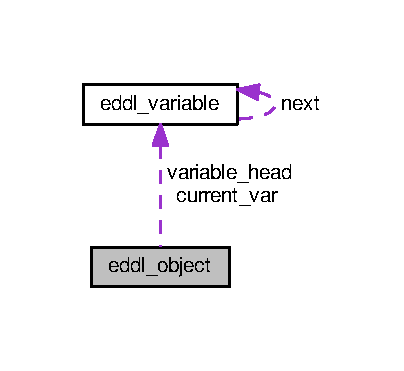
\includegraphics[width=194pt]{structeddl__object__coll__graph}
\end{center}
\end{figure}
\subsection*{Public Attributes}
\begin{DoxyCompactItemize}
\item 
int {\bfseries manufacturer}\hypertarget{structeddl__object_a068ca2f55a0ca714f6ae4081404ebcb8}{}\label{structeddl__object_a068ca2f55a0ca714f6ae4081404ebcb8}

\item 
uint16\+\_\+t {\bfseries device\+\_\+type}\hypertarget{structeddl__object_a011fbc1d6251efff7fc59e2e3862c3f8}{}\label{structeddl__object_a011fbc1d6251efff7fc59e2e3862c3f8}

\item 
int {\bfseries device\+\_\+revision}\hypertarget{structeddl__object_a0a81761adddc6f99ae2a9ed0203030c1}{}\label{structeddl__object_a0a81761adddc6f99ae2a9ed0203030c1}

\item 
int {\bfseries dd\+\_\+revision}\hypertarget{structeddl__object_a3194adb5ded71f027deae08e8add77bf}{}\label{structeddl__object_a3194adb5ded71f027deae08e8add77bf}

\item 
\hyperlink{structeddl__variable}{eddl\+\_\+variable\+\_\+t} $\ast$ {\bfseries current\+\_\+var}\hypertarget{structeddl__object_ac62753f0861985630e571401fa837268}{}\label{structeddl__object_ac62753f0861985630e571401fa837268}

\item 
\hyperlink{structeddl__variable}{eddl\+\_\+variable\+\_\+t} $\ast$ {\bfseries variable\+\_\+head}\hypertarget{structeddl__object_a0e174cf7f483bf8186502c7832cb682d}{}\label{structeddl__object_a0e174cf7f483bf8186502c7832cb682d}

\end{DoxyCompactItemize}


The documentation for this struct was generated from the following file\+:\begin{DoxyCompactItemize}
\item 
/home/alxhoff/git/\+E\+D\+D\+L-\/parser/\+E\+D\+D\+L-\/\+Parser/\hyperlink{eddl__data__type_8h}{eddl\+\_\+data\+\_\+type.\+h}\end{DoxyCompactItemize}

\hypertarget{structeddl__variable}{}\section{eddl\+\_\+variable Struct Reference}
\label{structeddl__variable}\index{eddl\+\_\+variable@{eddl\+\_\+variable}}


Collaboration diagram for eddl\+\_\+variable\+:\nopagebreak
\begin{figure}[H]
\begin{center}
\leavevmode
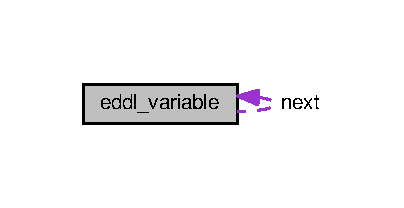
\includegraphics[width=194pt]{structeddl__variable__coll__graph}
\end{center}
\end{figure}
\subsection*{Public Attributes}
\begin{DoxyCompactItemize}
\item 
char $\ast$ {\bfseries \+\_\+\+\_\+name}\hypertarget{structeddl__variable_a79f72869d00e12136428752dfc7569d6}{}\label{structeddl__variable_a79f72869d00e12136428752dfc7569d6}

\item 
char $\ast$ {\bfseries \+\_\+\+\_\+label}\hypertarget{structeddl__variable_a548592853cc4e7a9430c3321407fca0a}{}\label{structeddl__variable_a548592853cc4e7a9430c3321407fca0a}

\item 
char $\ast$ {\bfseries \+\_\+\+\_\+help}\hypertarget{structeddl__variable_a235acfb1be68c32d2dee20eef45d0ff5}{}\label{structeddl__variable_a235acfb1be68c32d2dee20eef45d0ff5}

\item 
class\+\_\+mask\+\_\+t {\bfseries \+\_\+\+\_\+class}\hypertarget{structeddl__variable_a0364f90161275d87a06a162e64d74205}{}\label{structeddl__variable_a0364f90161275d87a06a162e64d74205}

\item 
type\+\_\+mask\+\_\+t {\bfseries \+\_\+\+\_\+type}\hypertarget{structeddl__variable_ada222428d7b8f70f69b6a429a03d881a}{}\label{structeddl__variable_ada222428d7b8f70f69b6a429a03d881a}

\item 
void $\ast$ {\bfseries \+\_\+\+\_\+default\+\_\+value}\hypertarget{structeddl__variable_a63447d16a05e098f3c24300b71a9aa85}{}\label{structeddl__variable_a63447d16a05e098f3c24300b71a9aa85}

\item 
handling\+\_\+mask\+\_\+t {\bfseries \+\_\+\+\_\+handling}\hypertarget{structeddl__variable_a4b412eb47c4a289a25a035a5dfe8e0fb}{}\label{structeddl__variable_a4b412eb47c4a289a25a035a5dfe8e0fb}

\item 
\hyperlink{structeddl__variable}{eddl\+\_\+variable\+\_\+t} $\ast$ {\bfseries next}\hypertarget{structeddl__variable_ade1f619bd50d2bea65354beef55fbd94}{}\label{structeddl__variable_ade1f619bd50d2bea65354beef55fbd94}

\end{DoxyCompactItemize}


The documentation for this struct was generated from the following file\+:\begin{DoxyCompactItemize}
\item 
/home/alxhoff/git/\+E\+D\+D\+L-\/parser/\+E\+D\+D\+L-\/\+Parser/\hyperlink{eddl__data__type_8h}{eddl\+\_\+data\+\_\+type.\+h}\end{DoxyCompactItemize}

\chapter{File Documentation}
\hypertarget{eddl__data__type_8h}{}\section{/home/alxhoff/git/\+E\+D\+D\+L-\/parser/\+E\+D\+D\+L-\/\+Parser/eddl\+\_\+data\+\_\+type.h File Reference}
\label{eddl__data__type_8h}\index{/home/alxhoff/git/\+E\+D\+D\+L-\/parser/\+E\+D\+D\+L-\/\+Parser/eddl\+\_\+data\+\_\+type.\+h@{/home/alxhoff/git/\+E\+D\+D\+L-\/parser/\+E\+D\+D\+L-\/\+Parser/eddl\+\_\+data\+\_\+type.\+h}}


Text parser to extract information from E\+DD files.  


{\ttfamily \#include \char`\"{}stdint.\+h\char`\"{}}\\*
Include dependency graph for eddl\+\_\+data\+\_\+type.\+h\+:
\nopagebreak
\begin{figure}[H]
\begin{center}
\leavevmode
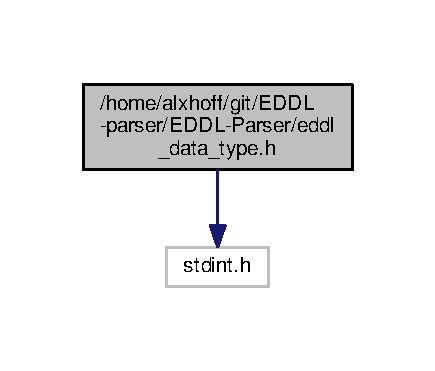
\includegraphics[width=209pt]{eddl__data__type_8h__incl}
\end{center}
\end{figure}
This graph shows which files directly or indirectly include this file\+:
\nopagebreak
\begin{figure}[H]
\begin{center}
\leavevmode
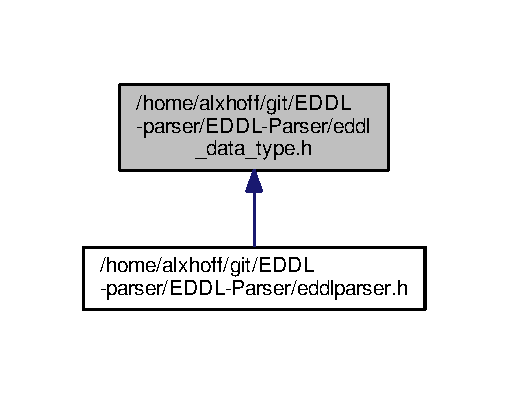
\includegraphics[width=244pt]{eddl__data__type_8h__dep__incl}
\end{center}
\end{figure}
\subsection*{Classes}
\begin{DoxyCompactItemize}
\item 
struct \hyperlink{structeddl__variable}{eddl\+\_\+variable}
\item 
struct \hyperlink{structeddl__object}{eddl\+\_\+object}
\end{DoxyCompactItemize}
\subsection*{Typedefs}
\begin{DoxyCompactItemize}
\item 
typedef struct \hyperlink{structeddl__variable}{eddl\+\_\+variable} {\bfseries eddl\+\_\+variable\+\_\+t}\hypertarget{eddl__data__type_8h_a6847bd33babd895988b46db909b45b6c}{}\label{eddl__data__type_8h_a6847bd33babd895988b46db909b45b6c}

\item 
typedef struct \hyperlink{structeddl__object}{eddl\+\_\+object} {\bfseries eddl\+\_\+object\+\_\+t}\hypertarget{eddl__data__type_8h_a2536096c229473a1ca4541d70a95950a}{}\label{eddl__data__type_8h_a2536096c229473a1ca4541d70a95950a}

\end{DoxyCompactItemize}
\subsection*{Enumerations}
\begin{DoxyCompactItemize}
\item 
enum {\bfseries E\+D\+D\+L\+\_\+\+P\+A\+R\+S\+E\+\_\+\+E\+R\+R\+\_\+t} \{ {\bfseries E\+D\+D\+L\+\_\+\+P\+A\+R\+S\+E\+\_\+\+OK}, 
{\bfseries E\+D\+D\+L\+\_\+\+P\+A\+R\+S\+E\+\_\+\+M\+EM}, 
{\bfseries E\+D\+D\+L\+\_\+\+P\+A\+R\+S\+E\+\_\+\+I\+N\+V\+AL}
 \}\hypertarget{eddl__data__type_8h_a1e2c9287866f8e37282d053234771e71}{}\label{eddl__data__type_8h_a1e2c9287866f8e37282d053234771e71}

\item 
enum {\bfseries class\+\_\+mask\+\_\+t} \{ {\bfseries I\+N\+V\+A\+L\+\_\+\+C\+L\+A\+S\+S\+\_\+e} = 0x00, 
{\bfseries C\+O\+N\+T\+A\+I\+N\+E\+D\+\_\+e} = 0x01, 
{\bfseries D\+Y\+N\+A\+M\+I\+C\+\_\+e} = 0x02
 \}\hypertarget{eddl__data__type_8h_a63528bdb3841a08895b345c700147706}{}\label{eddl__data__type_8h_a63528bdb3841a08895b345c700147706}

\item 
enum {\bfseries type\+\_\+mask\+\_\+t} \{ {\bfseries I\+N\+V\+A\+L\+\_\+\+T\+Y\+P\+E\+\_\+e} = 0x00, 
{\bfseries F\+L\+O\+A\+T\+\_\+e} = 0x01, 
{\bfseries I\+N\+T\+E\+G\+E\+R\+\_\+e} = 0x02
 \}\hypertarget{eddl__data__type_8h_a1169bd4ceba6bd82069ee94be7d2e9c8}{}\label{eddl__data__type_8h_a1169bd4ceba6bd82069ee94be7d2e9c8}

\item 
enum {\bfseries handling\+\_\+mask\+\_\+t} \{ {\bfseries I\+N\+V\+A\+L\+\_\+\+H\+A\+N\+D\+L\+E\+\_\+e} = 0x00, 
{\bfseries R\+E\+A\+D\+\_\+e} = 0x01, 
{\bfseries W\+R\+I\+T\+E\+\_\+e} = 0x02
 \}\hypertarget{eddl__data__type_8h_a90e82ce9e24299c257a801c8c50aeebe}{}\label{eddl__data__type_8h_a90e82ce9e24299c257a801c8c50aeebe}

\end{DoxyCompactItemize}


\subsection{Detailed Description}
Text parser to extract information from E\+DD files. 

\begin{DoxyAuthor}{Author}
Alex Hoffman 
\end{DoxyAuthor}
\begin{DoxyDate}{Date}
22 December 2017 
\end{DoxyDate}

\hypertarget{eddlparser_8h}{}\section{/home/alxhoff/git/\+E\+D\+D\+L-\/parser/\+E\+D\+D\+L-\/\+Parser/eddlparser.h File Reference}
\label{eddlparser_8h}\index{/home/alxhoff/git/\+E\+D\+D\+L-\/parser/\+E\+D\+D\+L-\/\+Parser/eddlparser.\+h@{/home/alxhoff/git/\+E\+D\+D\+L-\/parser/\+E\+D\+D\+L-\/\+Parser/eddlparser.\+h}}


Text parser to extract information from E\+DD files.  


{\ttfamily \#include \char`\"{}eddl\+\_\+data\+\_\+type.\+h\char`\"{}}\\*
Include dependency graph for eddlparser.\+h\+:
\nopagebreak
\begin{figure}[H]
\begin{center}
\leavevmode
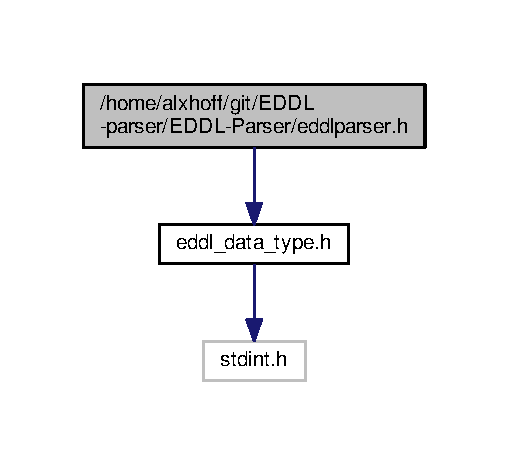
\includegraphics[width=244pt]{eddlparser_8h__incl}
\end{center}
\end{figure}
\subsection*{Functions}
\begin{DoxyCompactItemize}
\item 
\hyperlink{structeddl__object}{eddl\+\_\+object\+\_\+t} $\ast$ {\bfseries eddl\+\_\+parser\+\_\+create\+\_\+eddl\+\_\+t} (void)\hypertarget{eddlparser_8h_ab2aa5a789a88dd7feb93e9e250924cf1}{}\label{eddlparser_8h_ab2aa5a789a88dd7feb93e9e250924cf1}

\item 
E\+D\+D\+L\+\_\+\+P\+A\+R\+S\+E\+\_\+\+E\+R\+R\+\_\+t \hyperlink{eddlparser_8h_a6d13be0325fb446b19aecbed87d23e45}{eddl\+\_\+parser\+\_\+create\+\_\+variable\+\_\+t} (\hyperlink{structeddl__object}{eddl\+\_\+object\+\_\+t} $\ast$)
\item 
E\+D\+D\+L\+\_\+\+P\+A\+R\+S\+E\+\_\+\+E\+R\+R\+\_\+t \hyperlink{eddlparser_8h_a1cb28ff72b1c6d147aa30c715bd2fd1f}{eddl\+\_\+parser\+\_\+set\+\_\+manufacturer} (\hyperlink{structeddl__object}{eddl\+\_\+object\+\_\+t} $\ast$object, int val)
\item 
E\+D\+D\+L\+\_\+\+P\+A\+R\+S\+E\+\_\+\+E\+R\+R\+\_\+t \hyperlink{eddlparser_8h_addcca1c1db4becd183a0801a437fa26a}{eddl\+\_\+parser\+\_\+set\+\_\+device\+\_\+type} (\hyperlink{structeddl__object}{eddl\+\_\+object\+\_\+t} $\ast$object, long val)
\item 
E\+D\+D\+L\+\_\+\+P\+A\+R\+S\+E\+\_\+\+E\+R\+R\+\_\+t \hyperlink{eddlparser_8h_abddbe8f65af10fb75404d63efe4199be}{eddl\+\_\+parser\+\_\+set\+\_\+device\+\_\+revision} (\hyperlink{structeddl__object}{eddl\+\_\+object\+\_\+t} $\ast$object, int val)
\item 
E\+D\+D\+L\+\_\+\+P\+A\+R\+S\+E\+\_\+\+E\+R\+R\+\_\+t \hyperlink{eddlparser_8h_a6e47ee2ed39de45a84fc73d3122145cf}{eddl\+\_\+parser\+\_\+set\+\_\+dd\+\_\+revision} (\hyperlink{structeddl__object}{eddl\+\_\+object\+\_\+t} $\ast$object, int val)
\item 
E\+D\+D\+L\+\_\+\+P\+A\+R\+S\+E\+\_\+\+E\+R\+R\+\_\+t \hyperlink{eddlparser_8h_a34f2d73b4c545417c800892a680387cd}{eddl\+\_\+parser\+\_\+set\+\_\+variable\+\_\+name} (\hyperlink{structeddl__variable}{eddl\+\_\+variable\+\_\+t} $\ast$var, char $\ast$name)
\item 
E\+D\+D\+L\+\_\+\+P\+A\+R\+S\+E\+\_\+\+E\+R\+R\+\_\+t \hyperlink{eddlparser_8h_a4c6aca45070704667068f092dabf8fe2}{eddl\+\_\+parser\+\_\+set\+\_\+variable\+\_\+label} (\hyperlink{structeddl__variable}{eddl\+\_\+variable\+\_\+t} $\ast$var, char $\ast$label)
\item 
E\+D\+D\+L\+\_\+\+P\+A\+R\+S\+E\+\_\+\+E\+R\+R\+\_\+t \hyperlink{eddlparser_8h_aeb2728ab7d133eefa681203719e83113}{eddl\+\_\+parser\+\_\+set\+\_\+variable\+\_\+help} (\hyperlink{structeddl__variable}{eddl\+\_\+variable\+\_\+t} $\ast$var, char $\ast$help)
\item 
E\+D\+D\+L\+\_\+\+P\+A\+R\+S\+E\+\_\+\+E\+R\+R\+\_\+t \hyperlink{eddlparser_8h_a070f05bd34b6ec3f64c03bdbc9d6f04f}{eddl\+\_\+parser\+\_\+set\+\_\+variable\+\_\+class\+\_\+mask} (\hyperlink{structeddl__variable}{eddl\+\_\+variable\+\_\+t} $\ast$var, class\+\_\+mask\+\_\+t mask)
\item 
E\+D\+D\+L\+\_\+\+P\+A\+R\+S\+E\+\_\+\+E\+R\+R\+\_\+t \hyperlink{eddlparser_8h_a47d3e75c715447c056816fb3331287df}{eddl\+\_\+parser\+\_\+set\+\_\+variable\+\_\+type\+\_\+mask} (\hyperlink{structeddl__variable}{eddl\+\_\+variable\+\_\+t} $\ast$var, type\+\_\+mask\+\_\+t mask)
\item 
E\+D\+D\+L\+\_\+\+P\+A\+R\+S\+E\+\_\+\+E\+R\+R\+\_\+t \hyperlink{eddlparser_8h_a287b2a82ab939daeb8ff764fbb835419}{eddl\+\_\+parser\+\_\+set\+\_\+variable\+\_\+default\+\_\+value} (\hyperlink{structeddl__variable}{eddl\+\_\+variable\+\_\+t} $\ast$var, void $\ast$value)
\item 
E\+D\+D\+L\+\_\+\+P\+A\+R\+S\+E\+\_\+\+E\+R\+R\+\_\+t \hyperlink{eddlparser_8h_a0e0ec91ab7ac52eadb50e23cbd2b58bf}{eddl\+\_\+parser\+\_\+set\+\_\+variable\+\_\+handling} (\hyperlink{structeddl__variable}{eddl\+\_\+variable\+\_\+t} $\ast$var, handling\+\_\+mask\+\_\+t val)
\item 
class\+\_\+mask\+\_\+t \hyperlink{eddlparser_8h_a1ebd02936cb13804c88fcb828f34e3cd}{eddl\+\_\+parser\+\_\+get\+\_\+class\+\_\+mask} (char $\ast$class\+\_\+string)
\item 
type\+\_\+mask\+\_\+t \hyperlink{eddlparser_8h_a744b6d8e0e4c939d6148b4a01d14e275}{eddl\+\_\+parser\+\_\+get\+\_\+type\+\_\+mask} (char $\ast$type\+\_\+string)
\item 
handling\+\_\+mask\+\_\+t \hyperlink{eddlparser_8h_a9d1bea223f0f62e90c5aa8e626b68ebd}{eddl\+\_\+parser\+\_\+get\+\_\+handling\+\_\+mask} (char $\ast$handling\+\_\+string)
\item 
E\+D\+D\+L\+\_\+\+P\+A\+R\+S\+E\+\_\+\+E\+R\+R\+\_\+t \hyperlink{eddlparser_8h_a254d61aa68d2fa4a0a664690f41e8b80}{eddl\+\_\+parser\+\_\+print\+\_\+var} (\hyperlink{structeddl__variable}{eddl\+\_\+variable\+\_\+t} $\ast$var)
\end{DoxyCompactItemize}
\subsection*{Variables}
\begin{DoxyCompactItemize}
\item 
\hyperlink{structeddl__object}{eddl\+\_\+object\+\_\+t} $\ast$ {\bfseries doc\+\_\+object}\hypertarget{eddlparser_8h_ac32947cef301170b86bf2471f20b1117}{}\label{eddlparser_8h_ac32947cef301170b86bf2471f20b1117}

\end{DoxyCompactItemize}


\subsection{Detailed Description}
Text parser to extract information from E\+DD files. 

\begin{DoxyAuthor}{Author}
Alex Hoffman 
\end{DoxyAuthor}
\begin{DoxyDate}{Date}
22 December 2017 
\end{DoxyDate}


\subsection{Function Documentation}
\index{eddlparser.\+h@{eddlparser.\+h}!eddl\+\_\+parser\+\_\+create\+\_\+variable\+\_\+t@{eddl\+\_\+parser\+\_\+create\+\_\+variable\+\_\+t}}
\index{eddl\+\_\+parser\+\_\+create\+\_\+variable\+\_\+t@{eddl\+\_\+parser\+\_\+create\+\_\+variable\+\_\+t}!eddlparser.\+h@{eddlparser.\+h}}
\subsubsection[{\texorpdfstring{eddl\+\_\+parser\+\_\+create\+\_\+variable\+\_\+t(eddl\+\_\+object\+\_\+t $\ast$)}{eddl_parser_create_variable_t(eddl_object_t *)}}]{\setlength{\rightskip}{0pt plus 5cm}E\+D\+D\+L\+\_\+\+P\+A\+R\+S\+E\+\_\+\+E\+R\+R\+\_\+t eddl\+\_\+parser\+\_\+create\+\_\+variable\+\_\+t (
\begin{DoxyParamCaption}
\item[{{\bf eddl\+\_\+object\+\_\+t} $\ast$}]{}
\end{DoxyParamCaption}
)}\hypertarget{eddlparser_8h_a6d13be0325fb446b19aecbed87d23e45}{}\label{eddlparser_8h_a6d13be0325fb446b19aecbed87d23e45}

\begin{DoxyParams}{Parameters}
{\em } & \\
\hline
\end{DoxyParams}
\index{eddlparser.\+h@{eddlparser.\+h}!eddl\+\_\+parser\+\_\+get\+\_\+class\+\_\+mask@{eddl\+\_\+parser\+\_\+get\+\_\+class\+\_\+mask}}
\index{eddl\+\_\+parser\+\_\+get\+\_\+class\+\_\+mask@{eddl\+\_\+parser\+\_\+get\+\_\+class\+\_\+mask}!eddlparser.\+h@{eddlparser.\+h}}
\subsubsection[{\texorpdfstring{eddl\+\_\+parser\+\_\+get\+\_\+class\+\_\+mask(char $\ast$class\+\_\+string)}{eddl_parser_get_class_mask(char *class_string)}}]{\setlength{\rightskip}{0pt plus 5cm}class\+\_\+mask\+\_\+t eddl\+\_\+parser\+\_\+get\+\_\+class\+\_\+mask (
\begin{DoxyParamCaption}
\item[{char $\ast$}]{class\+\_\+string}
\end{DoxyParamCaption}
)}\hypertarget{eddlparser_8h_a1ebd02936cb13804c88fcb828f34e3cd}{}\label{eddlparser_8h_a1ebd02936cb13804c88fcb828f34e3cd}

\begin{DoxyParams}{Parameters}
{\em } & \\
\hline
\end{DoxyParams}
\index{eddlparser.\+h@{eddlparser.\+h}!eddl\+\_\+parser\+\_\+get\+\_\+handling\+\_\+mask@{eddl\+\_\+parser\+\_\+get\+\_\+handling\+\_\+mask}}
\index{eddl\+\_\+parser\+\_\+get\+\_\+handling\+\_\+mask@{eddl\+\_\+parser\+\_\+get\+\_\+handling\+\_\+mask}!eddlparser.\+h@{eddlparser.\+h}}
\subsubsection[{\texorpdfstring{eddl\+\_\+parser\+\_\+get\+\_\+handling\+\_\+mask(char $\ast$handling\+\_\+string)}{eddl_parser_get_handling_mask(char *handling_string)}}]{\setlength{\rightskip}{0pt plus 5cm}handling\+\_\+mask\+\_\+t eddl\+\_\+parser\+\_\+get\+\_\+handling\+\_\+mask (
\begin{DoxyParamCaption}
\item[{char $\ast$}]{handling\+\_\+string}
\end{DoxyParamCaption}
)}\hypertarget{eddlparser_8h_a9d1bea223f0f62e90c5aa8e626b68ebd}{}\label{eddlparser_8h_a9d1bea223f0f62e90c5aa8e626b68ebd}

\begin{DoxyParams}{Parameters}
{\em } & \\
\hline
\end{DoxyParams}
\index{eddlparser.\+h@{eddlparser.\+h}!eddl\+\_\+parser\+\_\+get\+\_\+type\+\_\+mask@{eddl\+\_\+parser\+\_\+get\+\_\+type\+\_\+mask}}
\index{eddl\+\_\+parser\+\_\+get\+\_\+type\+\_\+mask@{eddl\+\_\+parser\+\_\+get\+\_\+type\+\_\+mask}!eddlparser.\+h@{eddlparser.\+h}}
\subsubsection[{\texorpdfstring{eddl\+\_\+parser\+\_\+get\+\_\+type\+\_\+mask(char $\ast$type\+\_\+string)}{eddl_parser_get_type_mask(char *type_string)}}]{\setlength{\rightskip}{0pt plus 5cm}type\+\_\+mask\+\_\+t eddl\+\_\+parser\+\_\+get\+\_\+type\+\_\+mask (
\begin{DoxyParamCaption}
\item[{char $\ast$}]{type\+\_\+string}
\end{DoxyParamCaption}
)}\hypertarget{eddlparser_8h_a744b6d8e0e4c939d6148b4a01d14e275}{}\label{eddlparser_8h_a744b6d8e0e4c939d6148b4a01d14e275}

\begin{DoxyParams}{Parameters}
{\em } & \\
\hline
\end{DoxyParams}
\index{eddlparser.\+h@{eddlparser.\+h}!eddl\+\_\+parser\+\_\+print\+\_\+var@{eddl\+\_\+parser\+\_\+print\+\_\+var}}
\index{eddl\+\_\+parser\+\_\+print\+\_\+var@{eddl\+\_\+parser\+\_\+print\+\_\+var}!eddlparser.\+h@{eddlparser.\+h}}
\subsubsection[{\texorpdfstring{eddl\+\_\+parser\+\_\+print\+\_\+var(eddl\+\_\+variable\+\_\+t $\ast$var)}{eddl_parser_print_var(eddl_variable_t *var)}}]{\setlength{\rightskip}{0pt plus 5cm}E\+D\+D\+L\+\_\+\+P\+A\+R\+S\+E\+\_\+\+E\+R\+R\+\_\+t eddl\+\_\+parser\+\_\+print\+\_\+var (
\begin{DoxyParamCaption}
\item[{{\bf eddl\+\_\+variable\+\_\+t} $\ast$}]{var}
\end{DoxyParamCaption}
)}\hypertarget{eddlparser_8h_a254d61aa68d2fa4a0a664690f41e8b80}{}\label{eddlparser_8h_a254d61aa68d2fa4a0a664690f41e8b80}

\begin{DoxyParams}{Parameters}
{\em } & \\
\hline
\end{DoxyParams}
\index{eddlparser.\+h@{eddlparser.\+h}!eddl\+\_\+parser\+\_\+set\+\_\+dd\+\_\+revision@{eddl\+\_\+parser\+\_\+set\+\_\+dd\+\_\+revision}}
\index{eddl\+\_\+parser\+\_\+set\+\_\+dd\+\_\+revision@{eddl\+\_\+parser\+\_\+set\+\_\+dd\+\_\+revision}!eddlparser.\+h@{eddlparser.\+h}}
\subsubsection[{\texorpdfstring{eddl\+\_\+parser\+\_\+set\+\_\+dd\+\_\+revision(eddl\+\_\+object\+\_\+t $\ast$object, int val)}{eddl_parser_set_dd_revision(eddl_object_t *object, int val)}}]{\setlength{\rightskip}{0pt plus 5cm}E\+D\+D\+L\+\_\+\+P\+A\+R\+S\+E\+\_\+\+E\+R\+R\+\_\+t eddl\+\_\+parser\+\_\+set\+\_\+dd\+\_\+revision (
\begin{DoxyParamCaption}
\item[{{\bf eddl\+\_\+object\+\_\+t} $\ast$}]{object, }
\item[{int}]{val}
\end{DoxyParamCaption}
)}\hypertarget{eddlparser_8h_a6e47ee2ed39de45a84fc73d3122145cf}{}\label{eddlparser_8h_a6e47ee2ed39de45a84fc73d3122145cf}

\begin{DoxyParams}{Parameters}
{\em } & \\
\hline
\end{DoxyParams}
\index{eddlparser.\+h@{eddlparser.\+h}!eddl\+\_\+parser\+\_\+set\+\_\+device\+\_\+revision@{eddl\+\_\+parser\+\_\+set\+\_\+device\+\_\+revision}}
\index{eddl\+\_\+parser\+\_\+set\+\_\+device\+\_\+revision@{eddl\+\_\+parser\+\_\+set\+\_\+device\+\_\+revision}!eddlparser.\+h@{eddlparser.\+h}}
\subsubsection[{\texorpdfstring{eddl\+\_\+parser\+\_\+set\+\_\+device\+\_\+revision(eddl\+\_\+object\+\_\+t $\ast$object, int val)}{eddl_parser_set_device_revision(eddl_object_t *object, int val)}}]{\setlength{\rightskip}{0pt plus 5cm}E\+D\+D\+L\+\_\+\+P\+A\+R\+S\+E\+\_\+\+E\+R\+R\+\_\+t eddl\+\_\+parser\+\_\+set\+\_\+device\+\_\+revision (
\begin{DoxyParamCaption}
\item[{{\bf eddl\+\_\+object\+\_\+t} $\ast$}]{object, }
\item[{int}]{val}
\end{DoxyParamCaption}
)}\hypertarget{eddlparser_8h_abddbe8f65af10fb75404d63efe4199be}{}\label{eddlparser_8h_abddbe8f65af10fb75404d63efe4199be}

\begin{DoxyParams}{Parameters}
{\em } & \\
\hline
\end{DoxyParams}
\index{eddlparser.\+h@{eddlparser.\+h}!eddl\+\_\+parser\+\_\+set\+\_\+device\+\_\+type@{eddl\+\_\+parser\+\_\+set\+\_\+device\+\_\+type}}
\index{eddl\+\_\+parser\+\_\+set\+\_\+device\+\_\+type@{eddl\+\_\+parser\+\_\+set\+\_\+device\+\_\+type}!eddlparser.\+h@{eddlparser.\+h}}
\subsubsection[{\texorpdfstring{eddl\+\_\+parser\+\_\+set\+\_\+device\+\_\+type(eddl\+\_\+object\+\_\+t $\ast$object, long val)}{eddl_parser_set_device_type(eddl_object_t *object, long val)}}]{\setlength{\rightskip}{0pt plus 5cm}E\+D\+D\+L\+\_\+\+P\+A\+R\+S\+E\+\_\+\+E\+R\+R\+\_\+t eddl\+\_\+parser\+\_\+set\+\_\+device\+\_\+type (
\begin{DoxyParamCaption}
\item[{{\bf eddl\+\_\+object\+\_\+t} $\ast$}]{object, }
\item[{long}]{val}
\end{DoxyParamCaption}
)}\hypertarget{eddlparser_8h_addcca1c1db4becd183a0801a437fa26a}{}\label{eddlparser_8h_addcca1c1db4becd183a0801a437fa26a}

\begin{DoxyParams}{Parameters}
{\em } & \\
\hline
\end{DoxyParams}
\index{eddlparser.\+h@{eddlparser.\+h}!eddl\+\_\+parser\+\_\+set\+\_\+manufacturer@{eddl\+\_\+parser\+\_\+set\+\_\+manufacturer}}
\index{eddl\+\_\+parser\+\_\+set\+\_\+manufacturer@{eddl\+\_\+parser\+\_\+set\+\_\+manufacturer}!eddlparser.\+h@{eddlparser.\+h}}
\subsubsection[{\texorpdfstring{eddl\+\_\+parser\+\_\+set\+\_\+manufacturer(eddl\+\_\+object\+\_\+t $\ast$object, int val)}{eddl_parser_set_manufacturer(eddl_object_t *object, int val)}}]{\setlength{\rightskip}{0pt plus 5cm}E\+D\+D\+L\+\_\+\+P\+A\+R\+S\+E\+\_\+\+E\+R\+R\+\_\+t eddl\+\_\+parser\+\_\+set\+\_\+manufacturer (
\begin{DoxyParamCaption}
\item[{{\bf eddl\+\_\+object\+\_\+t} $\ast$}]{object, }
\item[{int}]{val}
\end{DoxyParamCaption}
)}\hypertarget{eddlparser_8h_a1cb28ff72b1c6d147aa30c715bd2fd1f}{}\label{eddlparser_8h_a1cb28ff72b1c6d147aa30c715bd2fd1f}

\begin{DoxyParams}{Parameters}
{\em } & \\
\hline
\end{DoxyParams}
\index{eddlparser.\+h@{eddlparser.\+h}!eddl\+\_\+parser\+\_\+set\+\_\+variable\+\_\+class\+\_\+mask@{eddl\+\_\+parser\+\_\+set\+\_\+variable\+\_\+class\+\_\+mask}}
\index{eddl\+\_\+parser\+\_\+set\+\_\+variable\+\_\+class\+\_\+mask@{eddl\+\_\+parser\+\_\+set\+\_\+variable\+\_\+class\+\_\+mask}!eddlparser.\+h@{eddlparser.\+h}}
\subsubsection[{\texorpdfstring{eddl\+\_\+parser\+\_\+set\+\_\+variable\+\_\+class\+\_\+mask(eddl\+\_\+variable\+\_\+t $\ast$var, class\+\_\+mask\+\_\+t mask)}{eddl_parser_set_variable_class_mask(eddl_variable_t *var, class_mask_t mask)}}]{\setlength{\rightskip}{0pt plus 5cm}E\+D\+D\+L\+\_\+\+P\+A\+R\+S\+E\+\_\+\+E\+R\+R\+\_\+t eddl\+\_\+parser\+\_\+set\+\_\+variable\+\_\+class\+\_\+mask (
\begin{DoxyParamCaption}
\item[{{\bf eddl\+\_\+variable\+\_\+t} $\ast$}]{var, }
\item[{class\+\_\+mask\+\_\+t}]{mask}
\end{DoxyParamCaption}
)}\hypertarget{eddlparser_8h_a070f05bd34b6ec3f64c03bdbc9d6f04f}{}\label{eddlparser_8h_a070f05bd34b6ec3f64c03bdbc9d6f04f}

\begin{DoxyParams}{Parameters}
{\em } & \\
\hline
\end{DoxyParams}
\index{eddlparser.\+h@{eddlparser.\+h}!eddl\+\_\+parser\+\_\+set\+\_\+variable\+\_\+default\+\_\+value@{eddl\+\_\+parser\+\_\+set\+\_\+variable\+\_\+default\+\_\+value}}
\index{eddl\+\_\+parser\+\_\+set\+\_\+variable\+\_\+default\+\_\+value@{eddl\+\_\+parser\+\_\+set\+\_\+variable\+\_\+default\+\_\+value}!eddlparser.\+h@{eddlparser.\+h}}
\subsubsection[{\texorpdfstring{eddl\+\_\+parser\+\_\+set\+\_\+variable\+\_\+default\+\_\+value(eddl\+\_\+variable\+\_\+t $\ast$var, void $\ast$value)}{eddl_parser_set_variable_default_value(eddl_variable_t *var, void *value)}}]{\setlength{\rightskip}{0pt plus 5cm}E\+D\+D\+L\+\_\+\+P\+A\+R\+S\+E\+\_\+\+E\+R\+R\+\_\+t eddl\+\_\+parser\+\_\+set\+\_\+variable\+\_\+default\+\_\+value (
\begin{DoxyParamCaption}
\item[{{\bf eddl\+\_\+variable\+\_\+t} $\ast$}]{var, }
\item[{void $\ast$}]{value}
\end{DoxyParamCaption}
)}\hypertarget{eddlparser_8h_a287b2a82ab939daeb8ff764fbb835419}{}\label{eddlparser_8h_a287b2a82ab939daeb8ff764fbb835419}

\begin{DoxyParams}{Parameters}
{\em } & \\
\hline
\end{DoxyParams}
\index{eddlparser.\+h@{eddlparser.\+h}!eddl\+\_\+parser\+\_\+set\+\_\+variable\+\_\+handling@{eddl\+\_\+parser\+\_\+set\+\_\+variable\+\_\+handling}}
\index{eddl\+\_\+parser\+\_\+set\+\_\+variable\+\_\+handling@{eddl\+\_\+parser\+\_\+set\+\_\+variable\+\_\+handling}!eddlparser.\+h@{eddlparser.\+h}}
\subsubsection[{\texorpdfstring{eddl\+\_\+parser\+\_\+set\+\_\+variable\+\_\+handling(eddl\+\_\+variable\+\_\+t $\ast$var, handling\+\_\+mask\+\_\+t val)}{eddl_parser_set_variable_handling(eddl_variable_t *var, handling_mask_t val)}}]{\setlength{\rightskip}{0pt plus 5cm}E\+D\+D\+L\+\_\+\+P\+A\+R\+S\+E\+\_\+\+E\+R\+R\+\_\+t eddl\+\_\+parser\+\_\+set\+\_\+variable\+\_\+handling (
\begin{DoxyParamCaption}
\item[{{\bf eddl\+\_\+variable\+\_\+t} $\ast$}]{var, }
\item[{handling\+\_\+mask\+\_\+t}]{val}
\end{DoxyParamCaption}
)}\hypertarget{eddlparser_8h_a0e0ec91ab7ac52eadb50e23cbd2b58bf}{}\label{eddlparser_8h_a0e0ec91ab7ac52eadb50e23cbd2b58bf}

\begin{DoxyParams}{Parameters}
{\em } & \\
\hline
\end{DoxyParams}
\index{eddlparser.\+h@{eddlparser.\+h}!eddl\+\_\+parser\+\_\+set\+\_\+variable\+\_\+help@{eddl\+\_\+parser\+\_\+set\+\_\+variable\+\_\+help}}
\index{eddl\+\_\+parser\+\_\+set\+\_\+variable\+\_\+help@{eddl\+\_\+parser\+\_\+set\+\_\+variable\+\_\+help}!eddlparser.\+h@{eddlparser.\+h}}
\subsubsection[{\texorpdfstring{eddl\+\_\+parser\+\_\+set\+\_\+variable\+\_\+help(eddl\+\_\+variable\+\_\+t $\ast$var, char $\ast$help)}{eddl_parser_set_variable_help(eddl_variable_t *var, char *help)}}]{\setlength{\rightskip}{0pt plus 5cm}E\+D\+D\+L\+\_\+\+P\+A\+R\+S\+E\+\_\+\+E\+R\+R\+\_\+t eddl\+\_\+parser\+\_\+set\+\_\+variable\+\_\+help (
\begin{DoxyParamCaption}
\item[{{\bf eddl\+\_\+variable\+\_\+t} $\ast$}]{var, }
\item[{char $\ast$}]{help}
\end{DoxyParamCaption}
)}\hypertarget{eddlparser_8h_aeb2728ab7d133eefa681203719e83113}{}\label{eddlparser_8h_aeb2728ab7d133eefa681203719e83113}

\begin{DoxyParams}{Parameters}
{\em } & \\
\hline
\end{DoxyParams}
\index{eddlparser.\+h@{eddlparser.\+h}!eddl\+\_\+parser\+\_\+set\+\_\+variable\+\_\+label@{eddl\+\_\+parser\+\_\+set\+\_\+variable\+\_\+label}}
\index{eddl\+\_\+parser\+\_\+set\+\_\+variable\+\_\+label@{eddl\+\_\+parser\+\_\+set\+\_\+variable\+\_\+label}!eddlparser.\+h@{eddlparser.\+h}}
\subsubsection[{\texorpdfstring{eddl\+\_\+parser\+\_\+set\+\_\+variable\+\_\+label(eddl\+\_\+variable\+\_\+t $\ast$var, char $\ast$label)}{eddl_parser_set_variable_label(eddl_variable_t *var, char *label)}}]{\setlength{\rightskip}{0pt plus 5cm}E\+D\+D\+L\+\_\+\+P\+A\+R\+S\+E\+\_\+\+E\+R\+R\+\_\+t eddl\+\_\+parser\+\_\+set\+\_\+variable\+\_\+label (
\begin{DoxyParamCaption}
\item[{{\bf eddl\+\_\+variable\+\_\+t} $\ast$}]{var, }
\item[{char $\ast$}]{label}
\end{DoxyParamCaption}
)}\hypertarget{eddlparser_8h_a4c6aca45070704667068f092dabf8fe2}{}\label{eddlparser_8h_a4c6aca45070704667068f092dabf8fe2}

\begin{DoxyParams}{Parameters}
{\em } & \\
\hline
\end{DoxyParams}
\index{eddlparser.\+h@{eddlparser.\+h}!eddl\+\_\+parser\+\_\+set\+\_\+variable\+\_\+name@{eddl\+\_\+parser\+\_\+set\+\_\+variable\+\_\+name}}
\index{eddl\+\_\+parser\+\_\+set\+\_\+variable\+\_\+name@{eddl\+\_\+parser\+\_\+set\+\_\+variable\+\_\+name}!eddlparser.\+h@{eddlparser.\+h}}
\subsubsection[{\texorpdfstring{eddl\+\_\+parser\+\_\+set\+\_\+variable\+\_\+name(eddl\+\_\+variable\+\_\+t $\ast$var, char $\ast$name)}{eddl_parser_set_variable_name(eddl_variable_t *var, char *name)}}]{\setlength{\rightskip}{0pt plus 5cm}E\+D\+D\+L\+\_\+\+P\+A\+R\+S\+E\+\_\+\+E\+R\+R\+\_\+t eddl\+\_\+parser\+\_\+set\+\_\+variable\+\_\+name (
\begin{DoxyParamCaption}
\item[{{\bf eddl\+\_\+variable\+\_\+t} $\ast$}]{var, }
\item[{char $\ast$}]{name}
\end{DoxyParamCaption}
)}\hypertarget{eddlparser_8h_a34f2d73b4c545417c800892a680387cd}{}\label{eddlparser_8h_a34f2d73b4c545417c800892a680387cd}

\begin{DoxyParams}{Parameters}
{\em } & \\
\hline
\end{DoxyParams}
\index{eddlparser.\+h@{eddlparser.\+h}!eddl\+\_\+parser\+\_\+set\+\_\+variable\+\_\+type\+\_\+mask@{eddl\+\_\+parser\+\_\+set\+\_\+variable\+\_\+type\+\_\+mask}}
\index{eddl\+\_\+parser\+\_\+set\+\_\+variable\+\_\+type\+\_\+mask@{eddl\+\_\+parser\+\_\+set\+\_\+variable\+\_\+type\+\_\+mask}!eddlparser.\+h@{eddlparser.\+h}}
\subsubsection[{\texorpdfstring{eddl\+\_\+parser\+\_\+set\+\_\+variable\+\_\+type\+\_\+mask(eddl\+\_\+variable\+\_\+t $\ast$var, type\+\_\+mask\+\_\+t mask)}{eddl_parser_set_variable_type_mask(eddl_variable_t *var, type_mask_t mask)}}]{\setlength{\rightskip}{0pt plus 5cm}E\+D\+D\+L\+\_\+\+P\+A\+R\+S\+E\+\_\+\+E\+R\+R\+\_\+t eddl\+\_\+parser\+\_\+set\+\_\+variable\+\_\+type\+\_\+mask (
\begin{DoxyParamCaption}
\item[{{\bf eddl\+\_\+variable\+\_\+t} $\ast$}]{var, }
\item[{type\+\_\+mask\+\_\+t}]{mask}
\end{DoxyParamCaption}
)}\hypertarget{eddlparser_8h_a47d3e75c715447c056816fb3331287df}{}\label{eddlparser_8h_a47d3e75c715447c056816fb3331287df}

\begin{DoxyParams}{Parameters}
{\em } & \\
\hline
\end{DoxyParams}

%--- End generated contents ---

% Index
\backmatter
\newpage
\phantomsection
\clearemptydoublepage
\addcontentsline{toc}{chapter}{Index}
\printindex

\end{document}
